\subsubsection{Workflow Package}
This package defines the logic behind the creation and the management of workflow templates, workflow instances and versions of workflow instances. It receives requests in the singleton object of WorkflowManager from the client application through the api package of the server application. The package also communicates with the database interface to safe and recall data aswell as with the API of Apache Airflow.

\class{WorkflowManager}

\begin{figure}[h]
\centerline{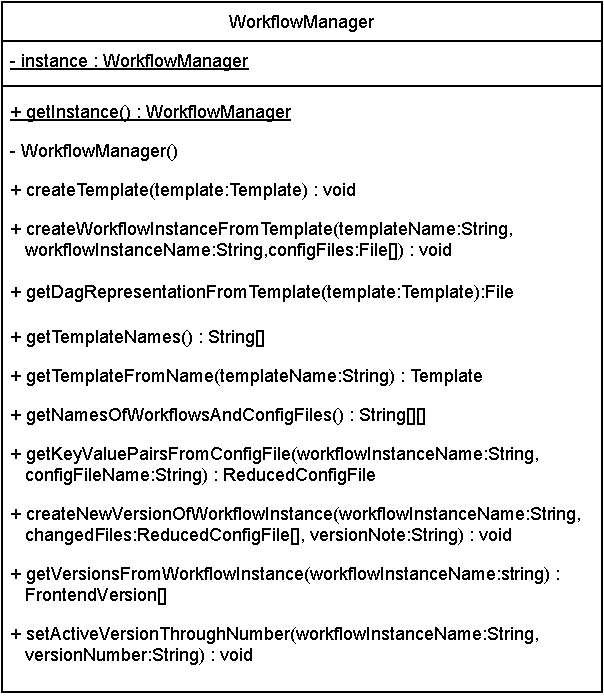
\includegraphics[scale=1]{res/Klassen/WorkflowManager.pdf}}
\caption{WorkflowManager class from class diagram}
\end{figure}

This class provides a singleton object that receives all requests addressed to this package. This class is also communicating with the API of Airflow as well as with the Database package.

\begin{methodenv}{Methods}

\method{getInstance():WorkflowManager}
Returns the singleton object if already existing otherwise it calls the private constructor

\method{createTemplate(template:Template):void}
Causes the creation of a new template entry in the database. The new template can be used for creating workflow instances afterwards.

\smallPara{Parameters}
\begin{itemize}
	\item{template:}
	A Template object that provides all the necessery components for creating a new workflow template
\end{itemize}

\smallPara{Exceptions}
\begin{itemize}
	\item{DoubleTemplateNameException}
	Gets thrown if the user trys to use an already existing template name
	\item{InvalidDagFileException}
	Gets thrown if the user hands over an invalid dag-definition-file
\end{itemize}

\method{createWorkflowInstanceFromTemplate(templateName:String, workflowInstanceName:String, configFiles:File[]):void}
Causes the instantiation of a workflow instance under the use of a workflow template. 

\smallPara{Parameters}
\begin{itemize}
	\item{templateName:}
	The identifier of the template that is used for instantiation
	\item{workflowInstanceName:}
	The name of the new workflow instance
	\item{configFiles:}
	Cointains all the files needed for the execution of the workflow
\end{itemize}

\smallPara{Exceptions}
\begin{itemize}
	\item{DoubleWorkflowInstanceNameException}
	Gets thrown if the user trys to use an already existing workflow instance name
	\item{EmptyConfigFolderException}
	Gets thrown if the user hands over an empty config-folder
\end{itemize}

\method{getTemplateNames():String[]}
Makes database request and returns the names of all templates in the system

\method{getTemplateFromName(templateName:String):Template}
Forwards the request for the named template to the database and returns result

\smallPara{Parameters}
\begin{itemize}
	\item{templateName:}
	The identifier of the desired template
\end{itemize}

\method{getNamesOfWorkflowsAndConfigFiles():String[][]}
Forwards the request to the database and returns the names of all workflow instances in combination with the associated config-files

\method{getKeyValuePairsFromConfigFile(workflowInstanceName:String, configFileName:String):String[][]}
Requests the desired config-file from the current version of the named workflow instance from the database. Afterwards changes the format from a file into an array of key-value-pairs and returns the result

\smallPara{Parameters}
\begin{itemize}
	\item{workflowInstanceName:}
	The identifier of the workflow instance
	\item{configFileName:}
	The name of the desired config file
\end{itemize}

\method{createNewVersionOfWorkflowInstance(workflowInstanceName:String, changedFiles:ReducedConfigFile[], versionNote:String):void}
Causes the creation of a new version of the workflow instance in the database. The predecessor of the new version is the active version of the instance.

\smallPara{Parameters}
\begin{itemize}
	\item{workflowInstanceName:}
	The identifier of the workflow instance of which a new version is created
	\item{changedFiles:}
	The config-files that were changed in comparison to the predecessor version in key-value-pair representation
	\item{versionNote}
	Note about the new version given by the user
\end{itemize}

\method{getVersionsFromWorkflowInstance(workflowInstanceName:string):FrontendVersion[]}
Requests information about all the versions of the given workflow instance from the database. Afterwards calculates the difference to the predecessor for every version and returns that information in combination with the version numbers and version notes

\smallPara{Parameters}
\begin{itemize}
	\item{workflowInstanceName:}
	The identifier of the given workflow instance
\end{itemize}

\method{setActiveVersionThroughNumber(workflowInstanceName:String, versionNumber:String):void}
Changes the active version of a workflow instance in the database

\smallPara{Parameters}
\begin{itemize}
	\item{workflowInstanceName:}
	The name of the workflow instance of which the active version shall be changed
	\item{versionNumber:}
	The number of the new active version
\end{itemize}

\smallPara{Exceptions}
\begin{itemize}
	\item{WorkflowInstanceRunningException}
	Gets thrown if the workflow instance is running. In that case the active version can not be changed
\end{itemize}
\end{methodenv}

%%%%%%%%%%%%%%%%%%%%%%%%%%%%%%%%%
\class{Template}

\begin{figure}[h]
\centerline{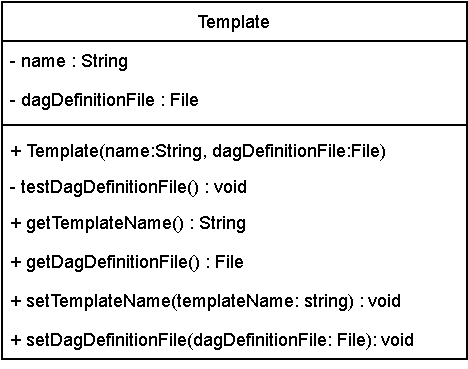
\includegraphics[scale=1]{res/Klassen/Template.pdf}}
\caption{Template class from class diagram}
\end{figure}

This class represents a workflow template. It contains the identifying name of the template as well as a dag-definition-file.

\begin{methodenv}{Constructor}

\method{Template(name:String, dagDefinitionFile:File):Template}

\smallPara{Parameters}
\begin{itemize}
	\item{name:}
	The name of the new template
	\item{dagDefinitionFile:}
	The file which defines the behavior of workflows instantiated of this template
\end{itemize}

\smallPara{Exceptions}
\begin{itemize}
	\item{DoubleTemplateNameException}
	Gets thrown if the database already contains a template with the given name
	\item{InvalidDagFileException}
	Gets thrown if the handed dag-definition-file is invalid
\end{itemize}
\end{methodenv}

%%%%%%%%%%%%%%%%%%%%%%%%%%%%%%

\class{WorkflowInstance}

\begin{figure}[h]
\centerline{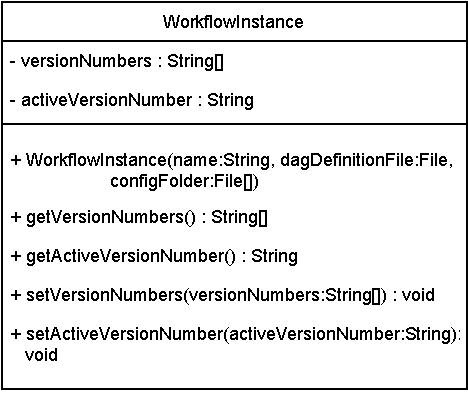
\includegraphics[scale=1]{res/Klassen/WorkflowInstance.pdf}}
\caption{WorkflowInstance class from class diagram}
\end{figure}

This class represents a workflow template. It contains the identifying name of the template as well as a dag-definition-file.

\begin{methodenv}{Constructor}

\method{WorkflowInstance(name:String, dagDefinitionFile:File, configFolder:File[]):WorkflowInstance}

\smallPara{Parameters}
\begin{itemize}
	\item{name:}
	The identifying name of the workflow instance
	\item{dagDefinitionFile:}
	The file which defines the behavior of the workflow instance
	\item{configFolder:}
	An array of files that is needed for executing the workflow
\end{itemize}

\smallPara{Exceptions}
\begin{itemize}
	\item{DoubleWorkflowInstanceNameException}
	Gets thrown if the workflow instance name is already given away to another workflow instance
	\item{EmptyConfigFolderException}
	Gets thrown if the handed configFolder-array is empty
\end{itemize}

\end{methodenv}

%%%%%%%%%%%%%%%%%%%%%%%%%%%%%%%%%

\class{ParameterChange}

\begin{figure}[h]
\centerline{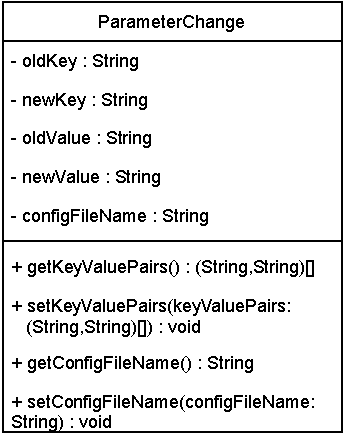
\includegraphics[scale=1]{res/Klassen/ParameterChange.pdf}}
\caption{ParameterChange class from class diagram}
\end{figure}

This class represents the change of a key-value pair. It contains the old aswell as the new version of both the key aswell as the value. Furthermore it holds the name of the file the change was made in.

\begin{methodenv}{Constructor}
\method{ParameterChange(oldKey:String, newKey:String, oldValue:String, newValue:String, configFileName:String):ParameterChange}
\smallPara{Parameters}
\begin{itemize}
	\item{oldKey:}
	The key of the pair before the change
	\item{newKey:}
	The key of the pair after the change
	\item{oldValue:}
	The value of the pair before the change
	\item{newValue:}
	The value of the pair after the change
	\item{configFileName:}
	The name of the file in which the change was made
\end{itemize}
\end{methodenv}

%%%%%%%%%%%%%%%%%%%%%%%%%%%%%%%%%

\class{ReducedConfigFile}

\begin{figure}[h]
\centerline{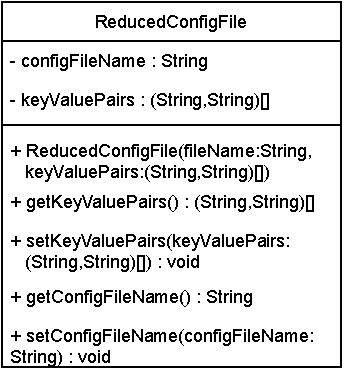
\includegraphics[scale=1]{res/Klassen/ReducedConfigFile.pdf}}
\caption{ReducedConfigFile class from class diagram}
\end{figure}

This class holds all information to represent a config-file in the frontend.

\begin{methodenv}{Constructor}

\method{ReducedConfigFile(fileName:String, keyValuePairs:(String,String)[]):ReducedConfigFile}

\smallPara{Parameters}
\begin{itemize}
	\item{fileName:}
	The name of the config-file through which the config-file can be identified among other config files of the workflow instance
	\item{keyValuePairs:}
	The contents of the file in key-value-pair representation
\end{itemize}
\end{methodenv}

%%%%%%%%%%%%%%%%%%%%%%%%%%%%%%%%%

\class{ConfigFile}

\begin{figure}[h]
\centerline{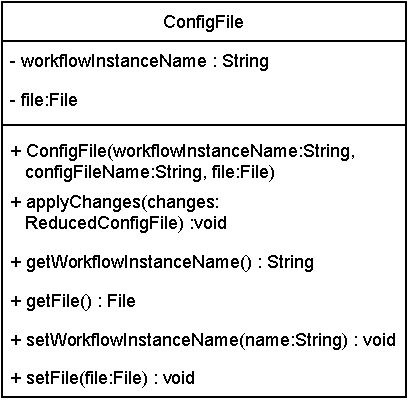
\includegraphics[scale=1]{res/Klassen/ConfigFile.pdf}}
\caption{ConfigFile class from class diagram}
\end{figure}

This is a subclass of ReducedConfigFile and additionally holds the config-file itself aswell as the name of the associated workflow instance.

\begin{methodenv}{Constructor}

\method{ConfigFile(workflowInstanceName:String, configFileName:String, file:File):ConfigFile}
It isn't necessary to hand the key-value-pairs because they can be derived from the file itself.

\smallPara{Parameters}
\begin{itemize}
	\item{workflowInstanceName:}
	The name of the associated workflow instance
	\item{configFileName:}
	The name of the config-file through which the config-file can be identified among other config files of the workflow instance
	\item{file:}
	The actual config-file
\end{itemize}
\end{methodenv}

\begin{methodenv}{Methods}


\method{applyChanges(changes:ReducedConfigFile):void}
The method compares the key-value-pairs given through the ReducedConfigFile to the pairs of the object itself. Changes detected are applied to the actual config file that is located in the database.

\smallPara{Parameters}
\begin{itemize}
	\item{changes:}
	Contains the key-value-pairs of the file after the changes made by the user in the frontend
\end{itemize}
\end{methodenv}

%%%%%%%%%%%%%%%%%%%%%%%%%%%%%%%%%

\class{Version}

\begin{figure}[h]
\centerline{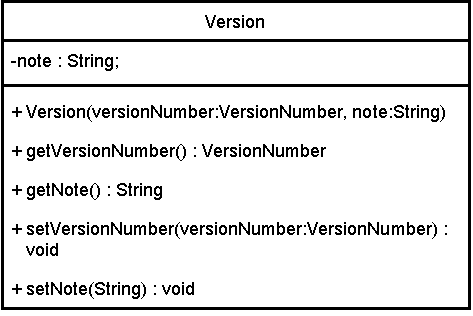
\includegraphics[scale=1]{res/Klassen/Version.pdf}}
\caption{Version class from class diagram}
\end{figure}

This class represents a version of a workflow instance. It's main task is to switch between the two different representations of versions one in the frontend, one in the database.
\begin{methodenv}{Constructor}


\method{Version(versionNumber:VersionNumber, note:String):Version}

\smallPara{Parameters}
\begin{itemize}
	\item{versionNumber:}
	Number that identifies the new Version
	\item{note:}
	Note from user that can be used for documenting the version
\end{itemize}
\end{methodenv}
%%%%%%%%%%%%%%%%%%%%%%%%%%%%%%%%%%%
\class{FrontendVersion}

\begin{figure}[h]
\centerline{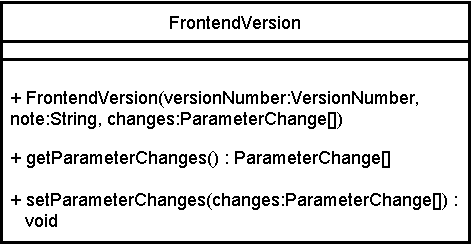
\includegraphics[scale=1]{res/Klassen/FrontendVersion.pdf}}
\caption{FrontendVersion class from class diagram}
\end{figure}

This class inherits from Version and is specialized to satisfy the need for information of the client application
\begin{methodenv}{Constructor}


\method{FrontendVersion(versionNumber:VersionNumber, note:String, changes:ParameterChange[]):FrontendVersion}

\smallPara{Parameters}
\begin{itemize}
	\item{versionNumber:}
	Number that identifies the new Version
	\item{note:}
	Note from user that can be used for documenting the version
	\item{changes:}
	Contains the difference to the predecessor version in form of the changed key-value-pairs
\end{itemize}
\end{methodenv}
%%%%%%%%%%%%%%%%%%%%%%%%%%%%%%%%%%%
\class{DatabaseVersion}

\begin{figure}[h]
\centerline{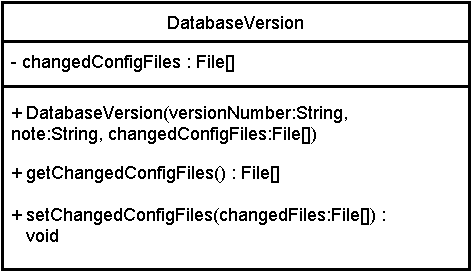
\includegraphics[scale=1]{res/Klassen/DatabaseVersion.pdf}}
\caption{DatabaseVersion class from class diagram}
\end{figure}

This class inherits from Version and is specialized to fit the way versions are managed in the database
\begin{methodenv}{Constructor}


\method{DatabaseVersion(versionNumber:VersionNumber, note:String, changedConfigFiles:File[]):DatabaseVersion}

\smallPara{Parameters}
\begin{itemize}
	\item{versionNumber:}
	Number that identifies the new Version
	\item{note:}
	Note from user that can be used for documenting the version
	\item{changedConfigFiles:}
	Contains all the config-files that were changed in this version
\end{itemize}
\end{methodenv}
%%%%%%%%%%%%%%%%%%%%%%%%%%%%%%%%%%%

\class{VersionNumber}

\begin{figure}[h]
\centerline{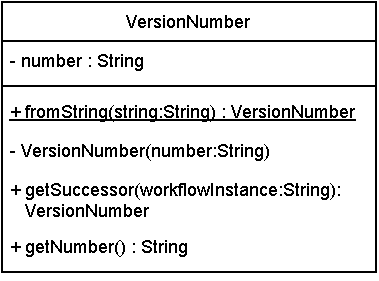
\includegraphics[scale=1]{res/Klassen/VersionNumber.pdf}}
\caption{VersionNumber class from class diagram}
\end{figure}

This class represents string expressions that are valid version numbers
\begin{methodenv}{Methods}

\method{static fromString(number:String):VersionNumber}
This static method converts a string of correct syntax into a VersionNumber by calling the private constructor.

\smallPara{Parameters}
\begin{itemize}
	\item{number:}
	String that has to fit the regular expression of a version number
\end{itemize}

\method{getSuccessor(workflowInstance:String):VersionNumber}
This method calculates the smallest free successor of the VersionNumber for the given workflow instance

\smallPara{Parameters}
\begin{itemize}
	\item{workflowInstance:}
	Identifier of the workflow instance to which the new number corresponds to
\end{itemize}
\end{methodenv}


%%%%%%%%%%%%%%%%%%%%%%%%%%%%%%%%%%%